\documentclass[9pt, oneside]{book}
\usepackage{xeCJK}
\usepackage{amsmath, amsthm, amssymb, bm, graphicx, hyperref, mathrsfs}
\usepackage{geometry}
% \geometry{b5paper,scale=0.85}
\geometry{b5paper,left=1.2cm,right=1.2cm,top=2cm,bottom=1cm}
\usepackage{graphicx} %插入图片的宏包
\usepackage{float} %设置图片浮动位置的宏包
\usepackage{subfigure} %插入多图时用子图显示的宏包
\usepackage{amstext} %公式中包含文字的宏包
\usepackage{booktabs} %插入表格的宏包
\usepackage{multirow} 
\usepackage{indentfirst} %设置缩进的宏包
\setlength{\parindent}{2em}
\usepackage{enumerate} %用于编号的宏包
\usepackage{hyperref} %用于引用的宏包
% \hypersetup{colorlinks, linkcolor=blue} %设置引用的字体颜色
\usepackage{color} %用于设置字体颜色的宏包
\usepackage{url} %用于超链接的宏包


% 封面部分
\title{\Huge{\textbf{ROS Notebook}}}
\author{Wu Yutian}
\date{2021.11.13}
\linespread{1.4}
\newtheorem{theorem}{定理}[section]
\newtheorem{definition}[theorem]{定义}
\newtheorem{lemma}[theorem]{引理}
\newtheorem{corollary}[theorem]{推论}
\newtheorem{example}[theorem]{例}
\newtheorem{proposition}[theorem]{命题}
\begin{document}

% 输出封面
\maketitle

% 前言部分
\pagenumbering{roman}
\setcounter{page}{1}

\begin{center}
    \Huge\textbf{前言}
\end{center}~\

\noindent{\large{本书的主要内容包括:}}
\normalsize
\begin{itemize}
    \item [-] 学习古月居的相关入门课程视频的内容记录
    \item [-] 阅读胡春旭的《ROS机器人开发实践》的笔记整理
    \item [-] 参考高翔的《视觉SLAM十四讲》补充了关于三维刚体运动学的内容
    \item [-] 参考一些博客阅读ros-navigation导航包源码的思路整理
    \item [-]
\end{itemize}

~\\
\begin{flushright}     
    \begin{tabular}{c}
        Wu Yutian\\
        2021.11.13
    \end{tabular}
\end{flushright}

\newpage
\pagenumbering{Roman}
\setcounter{page}{1}
\tableofcontents
\newpage
\setcounter{page}{1}
\pagenumbering{arabic}





\chapter{Navigation详细学习}

\section{global\_planner源码学习}

全局路径规划$BaseGlobalPlanner$的$plugin$有三种: $navfn/NavfnROS$,$global\_planner/GlobalPlanner$, $carrot\_planner/CarrotPlanner$. 其中常用的为$global\_planner/GlobalPlanner$,它是$navfn/NavfnROS$的改进版本,包含$Dijskstra$和$A*$算法进行全局路径规划。它与$Navfn$类似,也是提供了一个$makePlan$函数作为它被$move\_base$调用的总接口,负责实现全局的路径规划。


\subsection{$A^*$算法原理}

% 设$G=(V,E)$是一个带权有向图,把图中顶点集合$V$分成两组,第一组为已求出最短路径的顶点集合(用$S$表示,初始时$S$中只有一个源点,以后每求得一条最短路径 , 就将加入到集合$S$中,直到全部顶点都加入到$S$中,算法就结束了),第二组为其余未确定最短路径的顶点集合(用$U$表示),按最短路径长度的递增次序依次把第二组的顶点加入$S$中。在加入的过程中,总保持从源点$v$到$S$中各顶点的最短路径长度不大于从源点$v$到$U$中任何顶点的最短路径长度。此外,每个顶点对应一个距离,$S$中的顶点的距离就是从$v$到此顶点的最短路径长度,$U$中的顶点的距离,是从$v$到此顶点只包括$S$中的顶点为中间顶点的当前最短路径长度。

% 具体理解过程参照博客:

% \url{https://www.cnblogs.com/yutian-blogs/p/15605767.html}

\subsection{源码相关文件}

\begin{itemize}
    \item 源码链接:
    
    \url{https://github.com/ros-planning/navigation/tree/melodic-devel}

    \item 源码注释链接:
    
    \small
    \url{https://github.com/W-yt/ROS_Notes/tree/master/navigation-melodic-devel/global_planner}
    \normalsize
\end{itemize}

对应源码中的相关文件:

\begin{itemize}
    \item [-] global\_planner/src/plan\_node.cpp
    \item [-] global\_planner/src/planner\_core.cpp
    \item [-] global\_planner/src/astar.cpp
    \item [-] global\_planner/src/grid\_path.cpp
    \item [-] global\_planner/src/gradient\_path.cpp
    \item [-] global\_planner/include/potential\_calculator.h
    \item [-] global\_planner/src/quadratic\_calculator.cpp
    \item [-] global\_planner/include/expander.h
    \item [-] global\_planner/include/traceback.h
\end{itemize}

\subsection{整体结构图}

% \begin{figure}[H]
%     \centering
%     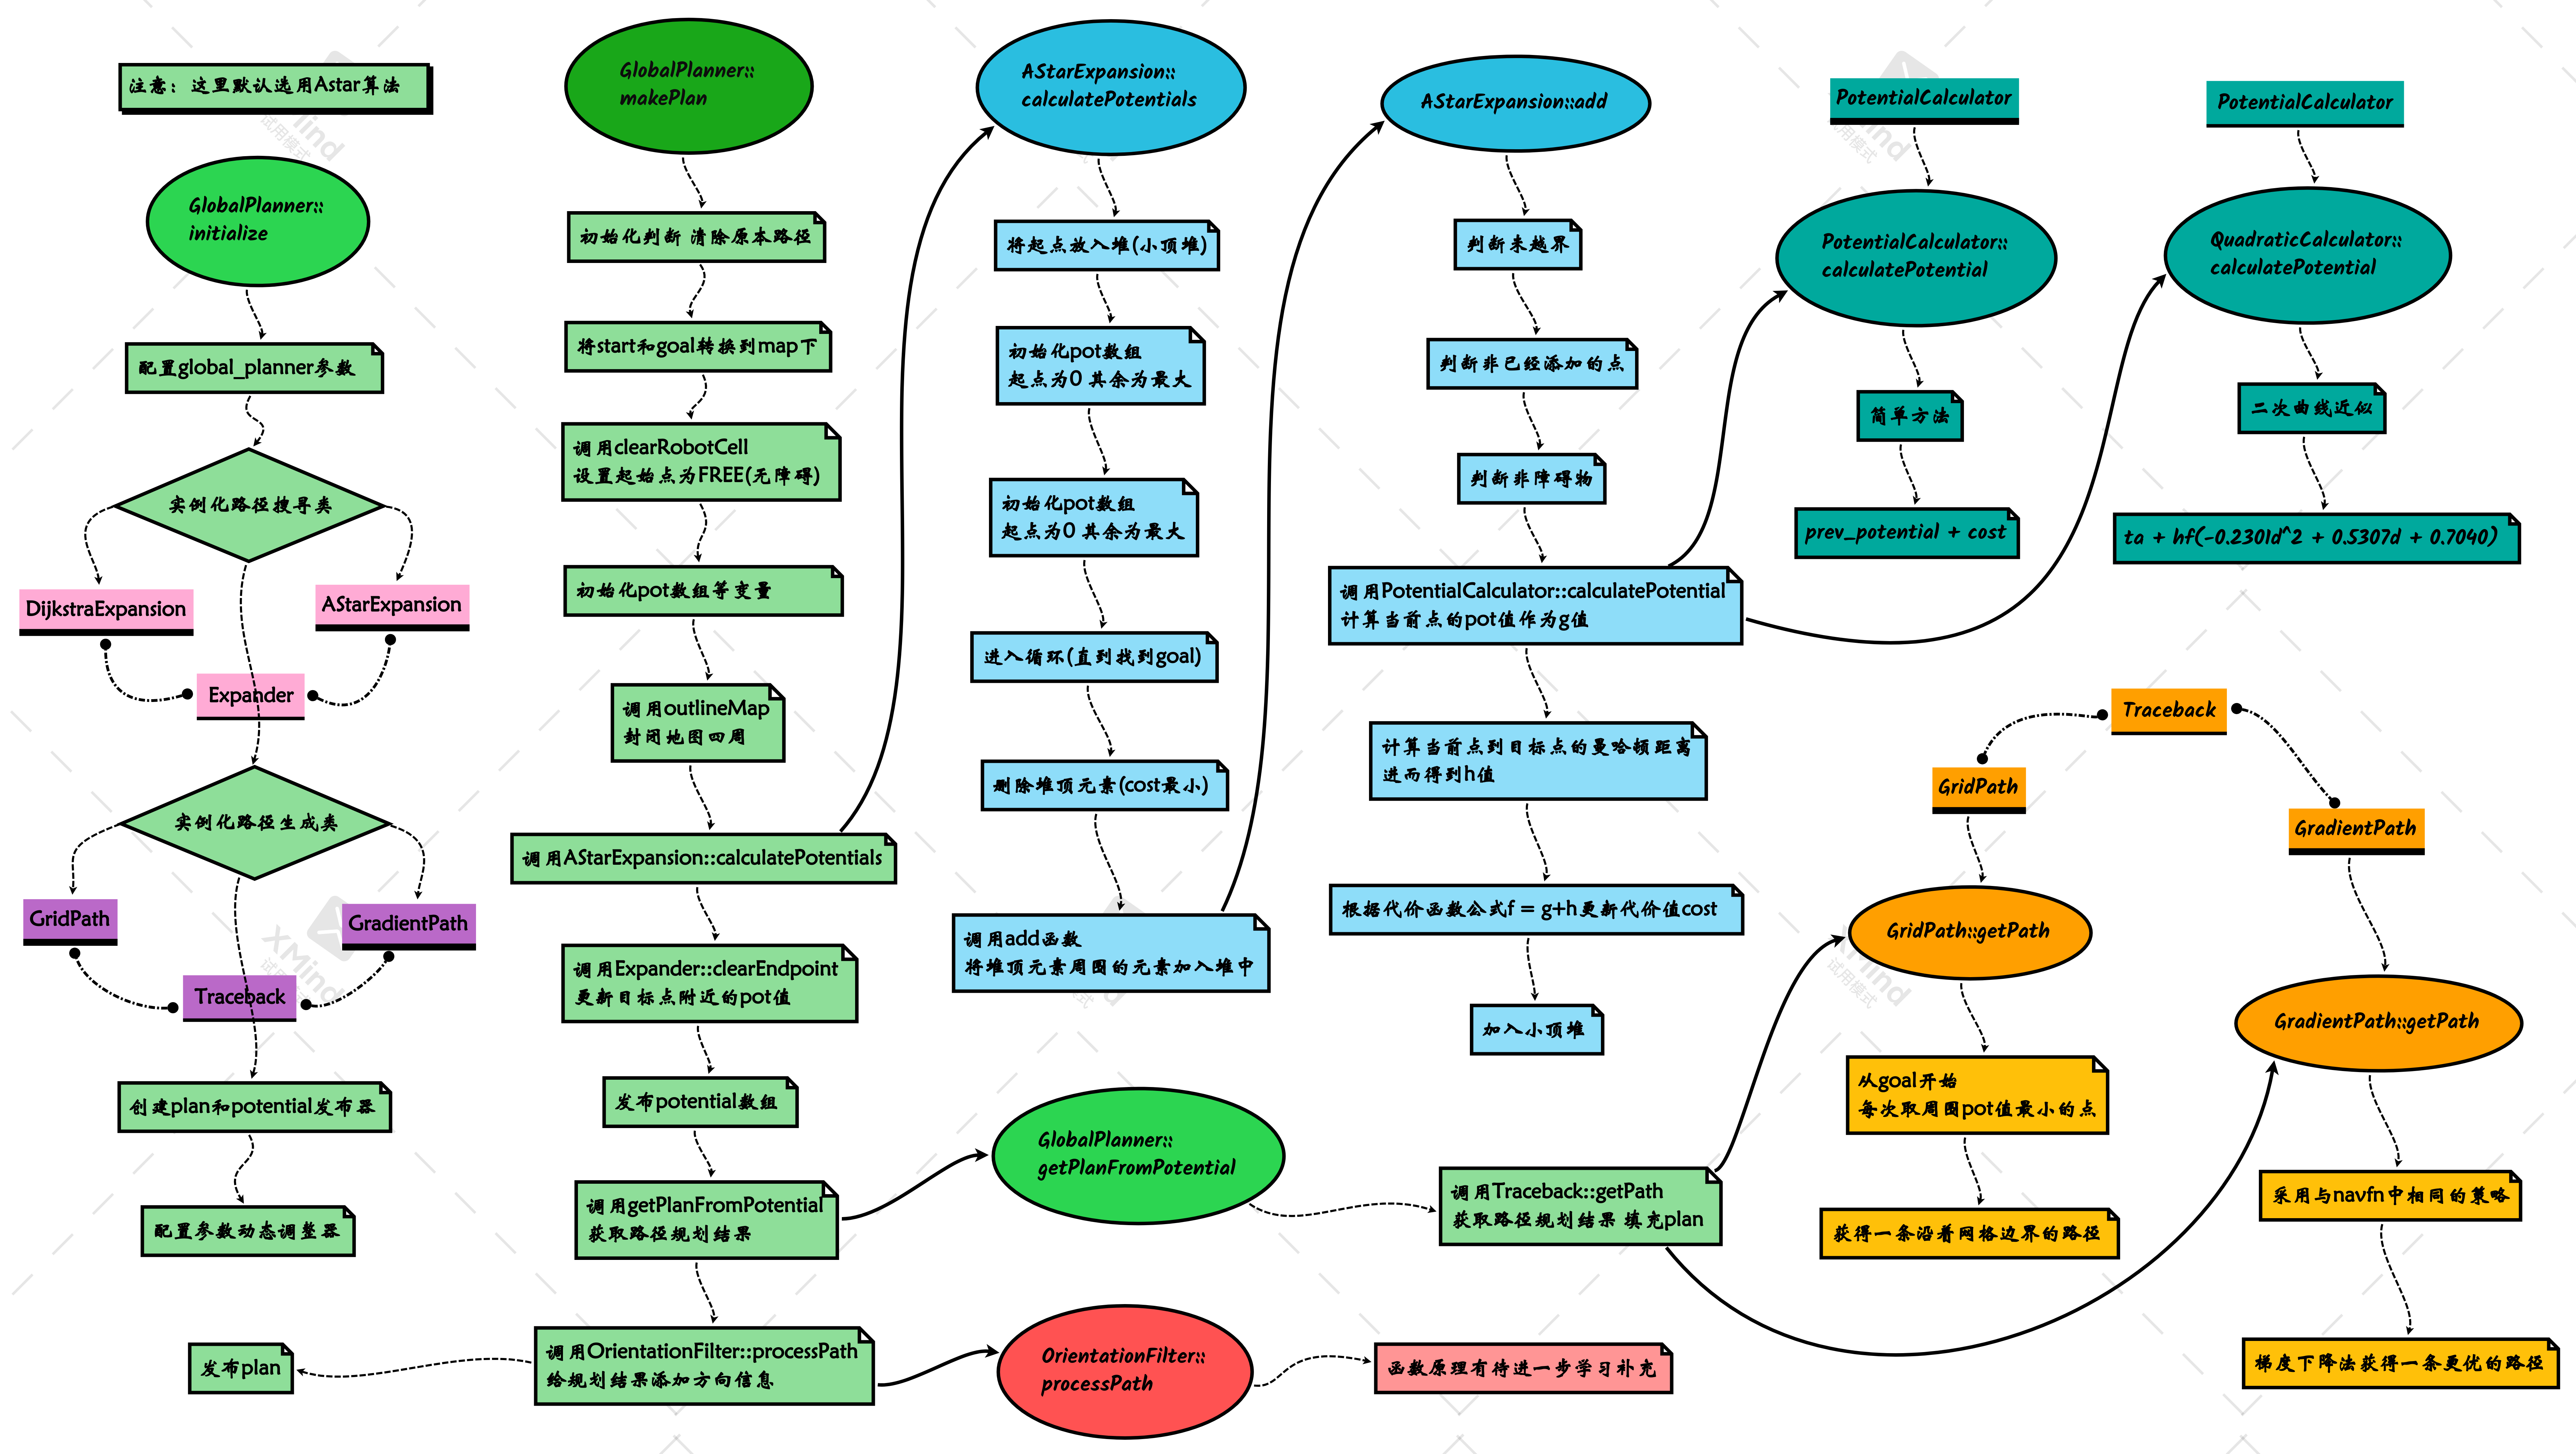
\includegraphics[width=1.0\linewidth]{image/global_planner.png}
% \end{figure}

\subsection{参数配置}

参数配置文件为:$global\_planner\_params.yaml$

参数列表:

\begin{itemize}
    \item [-] $allow\_unknown$:是否允许规划器规划穿过未知区域的路径(只设计该参数为$true$还不行,还要在$costmap\_commons\_params.yaml$中设置$track\_unknown\_space$参数也为$true$才行)
    \item [-] $default\_tolerance$:当设置的目的地被障碍物占据时,需要以该参数为半径寻找到最近的点作为新目的地点
    \item [-] $visualize\_potential$:是否显示从$PointCloud2$计算得到的势区域
    \item [-] $use\_dijkstra$:设置为$true$,将使用$dijkstra$算法,否则使用$A^*$算法
    \item [-] $use\_quadratic$:设置为$true$,将使用二次函数近似函数,否则使用更加简单的计算方式,这样节省硬件计算资源
    \item [-] $use\_grid\_path$:如果设置为$true$,则会规划一条沿着网格边界的路径,偏向于直线穿越网格,否则将使用梯度下降算法,路径更为光滑点
    \item [-] $old\_navfn\_behavior$:若在某些情况下,想让$global\_planner$完全复制$navfn$的功能,那就设置为$true$,但是需要注意$navfn$是非常旧的$ROS$系统中使用的,现在已经都用$global\_planne$r代替$navfn$了,所以不建议设置为$true$
    \item [-] $lethal\_cost$:致命代价值,默认是设置为253,可以动态来配置该参数
    \item [-] $neutral\_cost$:中等代价值,默认设置是50,可以动态配置该参数
    \item [-] $cost\_factor$:代价地图与每个代价值相乘的因子
    \item [-] $publish\_potential$:是否发布costmap的势函数
    \item [-] $orientation\_mode$:如何设置每个点的方向($None = 0,Forward = 1,Interpolate = 2,ForwardThenInterpolate = 3,Backward = 4,Leftward = 5,Rightward = 6$)(可动态重新配置)
    \item [-] $orientation\_window\_size$:根据$orientation\_mode$指定的位置积分来得到使用窗口的方向.默认值1,可以动态重新配置
\end{itemize}

\section{plan\_node.cpp}

$plan\_node.cpp$文件中是一个$PlannerWithCostmap$类,它继承自$GlobalPlanner$类(在$planner\_core$中定义)。在这个类中,主要开启了两个线程,提供了两种方式去开启$global\_planner$的规划,一种是服务请求,一种是发布目标goal话题。这部分在该类的构造函数中实现,代码如下:

\footnotesize
\begin{verbatim}
    PlannerWithCostmap::PlannerWithCostmap(string name, Costmap2DROS* cmap) :
            GlobalPlanner(name, cmap->getCostmap(), cmap->getGlobalFrameID()) {
        ros::NodeHandle private_nh("~");
        cmap_ = cmap;

        //第一个线程提供plan_service
        //一旦有请求,就调用bool success = makePlan(req.start, req.goal, path);
        make_plan_service_ = private_nh.advertiseService("make_plan", &PlannerWithCostmap::makePlanSer
    vice, this);

        //第二个线程是去订阅goal
        //拿到goal之后,就调用makePlan(start, *goal, path);
        pose_sub_ = private_nh.subscribe<rm::PoseStamped>("goal", 1, &PlannerWithCostmap::poseCallback, 
    this);
    }
\end{verbatim}
\normalsize

\subsection{planner\_core.cpp}

$planner\_core.cpp$文件是$global\_planner$的核心部分,包括了其中的$makePlan$函数,实现了全局路径规划的整体流程,相对与navfn的实现,代码更精简、封装更好,十分优雅。

\subsubsection{GlobalPlanner::initialize}

$GlobalPlanner$类的构造函数就是调用$initialize$函数,$initialize$函数中做了参数读取、功能包中用到的类的实例化,并且设置了参数动态配置。

\subsubsection{GlobalPlanner::makePlan}

该函数中包含了全局路径规划的整体流程逻辑,是该功能包的重点,代码逻辑与Navfn类似。

首先将目标点和起始点转换到$map$下,然后将起始点设置为$FREE$,并初始化$pot$数组,封闭地图四周,这些部分和$Navfn$相同,只是做了一层封装,用函数调用的方式实现。

接下来调用函数计算$potential$值,$planner\_$指针指向$A*$或$Dijkstrta$算法类 调用其各自的$calculatePotentials$函数,这是函数的重点,代码如下:

\small
\begin{verbatim}
    bool found_legal = planner_->calculatePotentials(costmap_->getCharMap(), 
                                                     start_x, start_y, goal_x, goal_y,
                                                     nx * ny * 2, potential_array_);

\end{verbatim}
\normalsize

接下来,如果在$calculatePotentials$中找到了合法的目标点,就可以获取规划的路径了,代码如下:

\small
\begin{verbatim}
    if (found_legal) {
        //根据pot数组获取路径规划结果plan(调用函数getPath 这个函数也有两种实现方式)
        if (getPlanFromPotential(start_x, start_y, goal_x, goal_y, goal, plan)) {
            //确保目标点和其余点有相同的时间戳
            geometry_msgs::PoseStamped goal_copy = goal;
            goal_copy.header.stamp = ros::Time::now();
            plan.push_back(goal_copy);
        } else {
            ROS_ERROR("Failed to get a plan from potential when a legal potential......");
        }
    }else{
        ROS_ERROR("Failed to get a plan.");
    }
\end{verbatim}
\normalsize

然后,给获得的路径数组添加方向信息,并发布规划结果,用于可视化:

\small
\begin{verbatim}
    //添加方向信息(给path“顺毛”保证拐弯的角度别变得太快)
    orientation_filter_->processPath(start, plan);
    //发布plan
    publishPlan(plan);
\end{verbatim}
\normalsize

\subsection{aster.cpp}

该文件中实现了$aster$路径搜索算法,实现方式简介优雅(与$Dijkstra$算法的复杂实现形成对比),值得借鉴。

需要注意:$A^*$ 算法是策略寻路,不保证一定是最短路径;$Dijkstra$ 算法是全局遍历,确保运算结果一定是最短路径,$Dijkstra$算法且算法需要载入全部数据,遍历搜索。

\subsubsection{AStarExpansion::calculatePotentials}

从起点开始逐渐扩散,将节点放入$open$堆,根据每个$cell$的代价值($cost$值)实现一个小顶堆。实现启发式搜索,不断计算更新经过的节点的$pot$值。

附带详细注释的代码如下:

\small
\begin{verbatim}
    bool AStarExpansion::calculatePotentials(unsigned char* costs, 
                                             double start_x, double start_y, 
                                             double end_x, double end_y,
                                             int cycles, float* potential) {
        //清空队列
        //queue_是启发式搜索到的向量队列<i,cost>
        queue_.clear();
        //toIndex函数获取索引值
        int start_i = toIndex(start_x, start_y);
        //将起点放入队列
        queue_.push_back(Index(start_i, 0));

        //std::fill:将一个区间的元素都赋予指定的值,即在(first, last)范围内填充指定值
        //将所有点的potential都设为一个极大值,potential就是估计值g,f=g+h
        //potential为g,也就是从起点到当前点的代价(Dijkstra算法中只有这个值)
        std::fill(potential, potential + ns_, POT_HIGH);
        //起点的potential值为0
        potential[start_i] = 0;

        //终点的索引
        int goal_i = toIndex(end_x, end_y);
        int cycle = 0;

        //循环目的:得到最小cost的索引,并删除它,如果索引指向goal则退出算法,返回true
        while (queue_.size() > 0 && cycle < cycles) {
            //将首元素放到最后,其他元素按照Cost值从小到大排列
            Index top = queue_[0];
            //pop_heap()是将堆顶元素与最后一个元素交换位置,之后用pop_back将最后一个元素删除
            //greate    
            r1()是自己定义的一个针对Index的比较函数,这里表示依据Index的小顶堆
            std::pop_heap(queue_.begin(), queue_.end(), greater1());
            queue_.pop_back();

            //小顶堆 所以top就是cost最小的点的索引
            int i = top.i;
            //如果到了目标点就结束
            if (i == goal_i)
                return true;

            //对前后左右四个点执行add函数,将代价最小点i周围点加入搜索队里并更新代价值
            add(costs, potential, potential[i], i + 1, end_x, end_y);
            add(costs, potential, potential[i], i - 1, end_x, end_y);
            add(costs, potential, potential[i], i + nx_, end_x, end_y);
            add(costs, potential, potential[i], i - nx_, end_x, end_y);

            cycle++;
        }
        return false;
    }
\end{verbatim}
\normalsize

\subsubsection{AStarExpansion::add}

该函数向$open$小顶堆中添加节点,并更新代价函数。如果是已经添加的点则忽略,根据$costmap$的值如果是障碍物的点也忽略。

更新代价函数的公式:

\begin{equation}
    f(n) = g(n) + h(n)
\end{equation}

其中,$g(n)$ 和 $h(n)$的意义见注释,代码如下:

\footnotesize
\begin{verbatim}
    void AStarExpansion::add(unsigned char* costs, 
                             float* potential, float prev_potential, 
                             int next_i, 
                             int end_x, int end_y) {
        //越界了
        if (next_i < 0 || next_i >= ns_)    return;

        //未搜索的点cost为POT_HIGH,如小于该值,则为已搜索点,跳过
        if (potential[next_i] < POT_HIGH)   return;

        //障碍物或者无信息的点
        if(costs[next_i]>=lethal_cost_ && 
           !(unknown_ && costs[next_i]==costmap_2d::NO_INFORMATION))
            return;
        
        //potential[next_i]是起点到当前点的cost即g(n)
        //prev_potentia是父节点的pot值
        potential[next_i] = p_calc_->calculatePotential(potential, costs[next_i] + neutral_cost_, next_i, 
    prev_potential);

        int x = next_i % nx_, y = next_i / nx_;
        //计算distance:从节点n到目标点最佳路径的估计代价,这里选用了曼哈顿距离(不能斜着走 且无视障碍物)
        float distance = abs(end_x - x) + abs(end_y - y);

        //distance只是格子个数,还有乘上每个格子的真实距离或是分辨率,所以最后h = distance*neutral_cost_
        //因此最后的f = h + g = potential[next_i] + distance*neutral_cost_
        //neutral_cost_默认值为50
        queue_.push_back(Index(next_i, potential[next_i] + distance * neutral_cost_));

        //插入小顶堆
        std::push_heap(queue_.begin(), queue_.end(), greater1());
    }
\end{verbatim}
\normalsize

\subsection{grid\_path.cpp}

因为如$A^*$算法已经完成了路径搜索的话,其实要获取路径只是需要从$goal$出发逆向走一遍就好了,所以这一部分要想实现很简单,但是这也只是一种简单的实现方式:创建一条沿着网格边界的路径;也可以采用梯度下降法,使用与$navfn$中相同的梯度下降算法实现方式(在$gradient\_path.cpp$中实现)。

getPath函数实现代码如下:

\small
\begin{verbatim}
    bool GridPath::getPath(float* potential, 
                           double start_x, double start_y, 
                           double end_x, double end_y, 
                           std::vector<std::pair<float, float> >& path) {
        //将goal的坐标放入current中
        std::pair<float, float> current;
        current.first = end_x;
        current.second = end_y;
    
        int start_index = getIndex(start_x, start_y);
    
        path.push_back(current);
        int c = 0;
        int ns = xs_ * ys_;
        
        while (getIndex(current.first, current.second) != start_index) {
            float min_val = 1e10;
            int min_x = 0, min_y = 0;
            //从周围的8个点中寻找pot值最小的点
            for (int xd = -1; xd <= 1; xd++) {
                for (int yd = -1; yd <= 1; yd++) {
                    if (xd == 0 && yd == 0)
                        continue;
                    int x = current.first + xd, y = current.second + yd;
                    int index = getIndex(x, y);
                    if (potential[index] < min_val) {
                        min_val = potential[index];
                        min_x = x;
                        min_y = y;
                    }
                }
            }
            if(min_x == 0 && min_y == 0)
                return false;
            current.first = min_x;
            current.second = min_y;
            path.push_back(current);
            
            //设置了一个循环次数的上限
            if(c++ > ns*4){
                return false;
            }
    
        }
        return true;
    }    
\end{verbatim}
\normalsize

\subsection{gradient\_path.cpp}

梯度下降算法实现路径获取的实现方式,与$navfn$中的实现相同,不再赘述。

\subsection{potential\_calculator.h}

$calculatePotential()$计算根据$use\_quadratic$的值有下面两个选择:

该函数计算pot值。

\begin{itemize}
    \item [-] 若为True  则使用二次曲线计算
    \item [-] 若为False 则采用简单方法计算
\end{itemize}

简单方法即直接返回如下算式: 

\begin{equation}
    \begin{aligned}
        new pot &= prev\_potential + cost\\
                &= prev\_potential + costs[next\_i] + neutral\_cost\_\\
                &= \mbox{之前路径代价g} + \mbox{地图代价} + \mbox{单格距离代价(初始化为50)}
    \end{aligned}
\end{equation}

代码如下:

\small
\begin{verbatim}
    virtual float calculatePotential(float* potential, unsigned char cost, int n, float prev_po
tential=-1){
        //如果父节点的pot值小于0(调用时没有赋值 使用了缺省值-1)
        //(在函数clearEndpoint中会出现这种缺省调用的情况)
        if(prev_potential < 0){
            //则将周围四个点的pot的最小值当做父节点的pot值
            float min_h = std::min(potential[n - 1], potential[n + 1]);
            float min_v = std::min(potential[n - nx_], potential[n + nx_]);
            prev_potential = std::min(min_h, min_v);
        }

        return prev_potential + cost;
    }
\end{verbatim}
\normalsize

其实实现的代码就是直接$return$就好了,但是为了适配$clearEndpoint$函数也可以直接调用,设置了缺省值,添加了上面的部分。

\subsection{quadratic\_calculator.cpp}

该函数计算pot值,采用了与navfn中相同的二次曲线的计算方法,不再赘述。

\subsection{expander.h}

这个文件中定义了$Expander$类,这是两个路径搜索算法($astar$和$dijkstra$)的父类,如果想要自己实现一个路径搜索算法也可以考虑继承该类。具体代码没有什么内容,不再介绍。

\subsection{traceback.h}

这个文件中定义了$Tracebac$k类,这是两个路径获取算法($grid\_path$和$gradient\_path$)的父类,如果想要自己实现一个路径获取算法也可以考虑继承该类。具体代码没有什么内容,不再介绍。


\end{document}